
\section{Object Registration}
\label{sec:region_registration}

From the segmentation stage described in Sec.~\ref{sec:segmentation}, we get a set of object regions, $\{R_{i,k}\}_{i=1,\ldots,n_k;k=1,\ldots,K}$, in the RGBD images.
Once we have the correspondences between regions in different frames, we can build geometric object models by rigid registration. 
However, it is non-trivial to recover the correspondence due to the imperfect segmentation.
One object maybe segmented into more than one regions while two objects maybe in the same region due to their similar appearance and close to each other. 


Recovering correspondence is to compute a set of object classes $\{C_{l}\}^N_{l=1}$ from all the regions. However, \redemph{the difficulty} is the total number of all the object classes $N$ is unknown, and the total number of regions $\sum_{k=1}^{K} n_k$ is very large so that it is non-trivial to compute the correspondences between all the RGBD images in a long time.
On the other hand, objects appear or disappear in the entire time period so that the total numbers of object instances $n_k$ in each frame are not the same. It brings more challenges. 



In order to solve the problem with \redemph{unknown number of object classes} and \redemph{unknown number of instances} in each frame, we use a three-level decision tree to cluster rgbd regions using appearance features and geometric features, respectively. 
As Figure~\ref{fig:object_decision_tree} shows,
given all the rgbd region without any correspondences, we first cluster the regions into foreground/background. 
Then we cluster foreground regions according to color histogram features. Then for each set of regions with similar appearance, we cluster them then by geometric features.  

\begin{figure}
	\centering
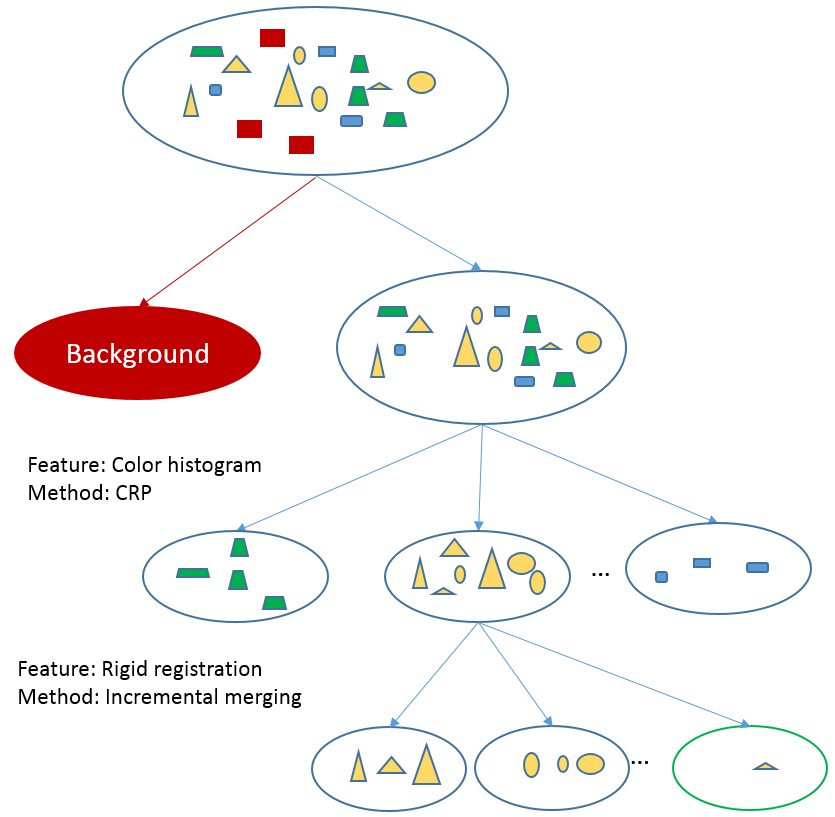
\includegraphics[width=\columnwidth]{figures/regions2objects.png}
\caption{A decision tree to cluster image regions into objects.}
\label{fig:object_decision_tree}
\end{figure}

\comment{
For each RGBD segment $S_{i}$, we compute its features $\vb{x}_i$ including
\begin{enumerate}
	\item The appearance features $\vb{h}^a_{i}$: include a typical Bag of Words (BoW) image representation. The length of the codebook is $100$.
	\item Geometric features  $\vb{h}^d_i$: a typical BoW of the depth image;
	\item the size $\vb{s}_i$ of the segment;
	\item $h_i$: the height of the object where it stands;
	\item $\vb{h}_i^n$: the normal histogram with 16 bins. 
\end{enumerate}
}



\subsection{Clustering regions via appearance features}

We use a non-parametric Bayesian modeling based on Dirichlet process to solve the clustering problem with unknown number of clusters. More specially, our problem can be formulated in a framework of distance dependent Chinese Restaurant Processes~(ddCRP)~\cite{ddCRPBlei}\cite{walon13cvpr}. 


\subsubsection{ddCRP}
 
CRP is an alternative representation of Dirichlet process model and it defines the following procedure. Imagine a restaurant with an infinite number of tables. A sequence of customers come enter the restaurant and sit at randomly chosen tables. The i-th customer sits down at a table with a probability that is proportional to how many customers are already sitting at that table or opens up a new table with a probability proportional to a hyperparameter. Their seating configuation represents a random partition also called \emph{table assignments}. Thus CRP provides a flexible prior distribution over table assignments where the number of tables is potentially infinite. 
Since the table assignment of each customer just depends on the number of people sitting at each table and is independent of the other ones, the ordering of customers does not affect the distribution over partitions and therefore exchangeability holds. 


While in some cases there are spatial or temporal dependencies between customers, the exchangeability does not hold any more, the generalized process allowing nonexchangeable distribution over partitions is needed. The ddCRP was proposed to offer an intuitive way for modeling non-exchangeability and dependency. The main difference between the CRP and ddCRP is that rather than directly linking customers to tables with table assignments, in ddCRP customers sit down with other customers according to the dependencies between them, which leads to customer assignments. Groups of customers sit together at a table only implicitly if they can be connected by traversing the customer assignments. Therefore the $i$-th customer sits with customer $j$ with a probability inversely proportional to the distance $d_{ij}$ between them or sits alone with a probability proportional to the hyperparameter $\alpha$:

\begin{equation}
p(c_i=j|D,f,\alpha) \propto \left \{ 
\begin{array}{ll}
f(d_{ij}) & j \neq i \\
\alpha    & j = i   
\end{array}
\right.
\label{eq:ddCRP}
\end{equation}
%
where $c_i$ is the customer assignment for customer $i$, and $f(d)$ is the decay function, and $D$ denotes the set of all distances between customers. 
The decay function $f$ should be non-increasing, takes non-negative finite values, and satisfies $f(\infty) = 0$. 
It describes how distances between customers affect the probabilities of linking them together.

\comment{ 
Figure~\ref{fig:ddCRP} demonstrates a ddCRP, from which we can see how to cluster the customer to different clusters/tables with unknown number of clusters. 


\begin{figure}
\centering
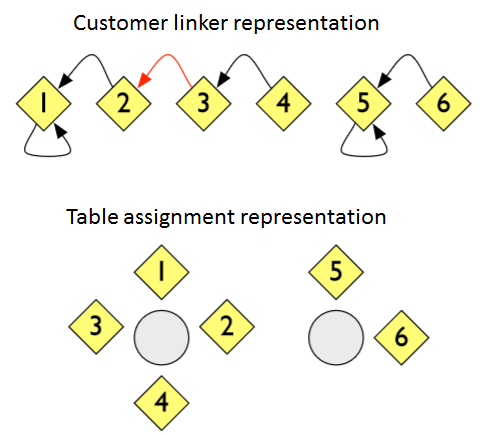
\includegraphics[width=\columnwidth]{figures/ddCRP.png}
\caption{Illustration of a ddCRP. For each customer $i$ (yellow square), ddCRP assigns another customer $j$ for him to sit with (upper). The table assignment (bottom) can be derived from the customer linker. }
\label{fig:ddCRP}
\end{figure}
}

\subsection{Region clustering using ddCRP}

Given a set of foreground RGBD regions $R_i$, we cluster them into classes $C_l$ using ddCRP based on appearance feature, like color histogram using HSV, as following:
\begin{algorithm}[htb]
\caption{Region clustering using ddCRP}
\begin{algorithmic}[1]
\REQUIRE ~~\\
A set of rgbd regions $\mathcal{R}=\{R_i\}_{i=1,\ldots,N}$;
\ENSURE ~~\\
A set of object clustering $\mathcal{C}=\{C_j\}_{j=1,\ldots,M}$;
\STATE $M=0$;
\FOR {$i=1$; $i<N$; ++$i$}
\FOR {$j=1$; $j<i$; ++$j$}
\STATE Compute similarity of $sim_{i,j}$;
\IF {$sim_{i,j}>T_{crp}$}
\STATE Assign same label: $l(R_i)=l(R_j)$;
\STATE break;
\ENDIF
\ENDFOR
\ENDFOR
\IF {$j==i$} 
\STATE $//$ No similar region is found for $R_i$, assign $R_i$ as a new object;
\STATE $M=M+1$;
\STATE $l(R_i)=M$;
\ENDIF
\end{algorithmic}
\end{algorithm}



Figure~\ref{fig:ddcrp_color_histogram} illustrates the process of assigning tables/classes using pairwise similarity. We can see that color histogram is effective to cluster image regions with similar appearance together. 
Due the color feature is not distinguished enough, regions have similar appearance are assigned to the same object. However, they have very different geometry features. 
For example, the large sofa and the two short sofas are assigned to the same group because their appearances are very similar. Therefore, we further split the clusters into different objects by geometric features. 
	

\begin{figure}
	\centering
	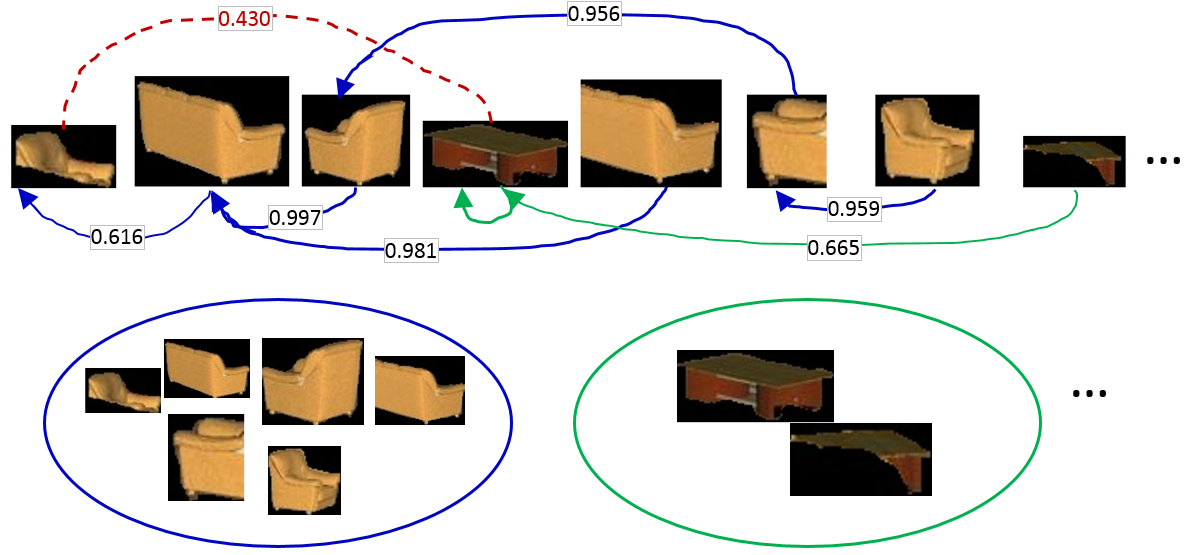
\includegraphics[width=\columnwidth]{figures/crp_ch.png}
	\caption{	\label{fig:ddcrp_color_histogram} Merging regions in to objects. By assigning object labels for all regions progressively, we can cluster the eight sofa regions into two object classes by color histograms. Solid lines indicate the same object label for the two regions. Dash lines indicate that for current region, the largest similarities with previous regions is lower than the threshold. Different colors indicate different object groups. }
\end{figure}


\subsection{Clustering objects by rigid registration}
%
Geometric features are usually accurate to judge if two regions are from the same object.
However, it usually takes much more time than comparing color histogram. 
%
One option is to compute pair-wise registration error between all the segments and then run a clustering process to group segments that from the same object. 
However, rigid registration brings large computing load to the process.
%
In order to facilitate the clustering process, we present a cascade method to efficiently cluster the regions and generate object models, as described in Algorithm~\ref{alg:region_registration}.

\begin{algorithm}
\caption{Clustering regions by rigid registration.}
\begin{algorithmic}
\REQUIRE ~~\\
A set of rgbd regions $\mathcal{R}=\{R_i\}_{i=1,\ldots,N}$ with similar appearance;
\ENSURE ~~\\
A set of object clustering $\mathcal{C}=\{C_j\}_{j=1,\ldots,M}$;
\STATE Initialization: $\mathcal{C}=\Phi$, $M=1$; \label{step:initialization_object}
\STATE Sorting the regions by size in decreasing order;
\WHILE {$\mathcal{R} \neq \Phi$}
\FOR {each object class $C_j$ in $\mathcal{C}$}
\STATE Clear the list $L_j$ of new regions for object $C_j$
\FOR {each region $R_i$ in $\mathcal{R}$}
\STATE Register $R_i$ with $C_j$ in a lower resolution;
\IF {$E^1_{fit}(R_i,C_j) < T^1_{reg}$} 
\STATE $//$ Quickly select the region that is similar enough;
\STATE Register $R_i$ with $C_j$ in a higher resolution;
\IF   {$E^2_{fit}(R_i,C_j) < T^2_{reg}$} 
\STATE Add $R_i$ to the candidate region list $L_j$ 
\ENDIF
\ENDIF
\ENDFOR %end for register region to object_j
\STATE Select the region $R^*$ with minimum registration error $E^2_{fit}$;
\STATE Update object $C_i$ with $R^*$;
\STATE Mark $R^*$ as "merged"; Mark $C_i$ as "updated";
\ENDFOR % end for all regions
\IF {At least one region is "merged"}
\STATE Remove all the "merged" regions;
\ELSE
\STATE Add the largest region in $\mathcal{R}$ as a new object into $\mathcal{C}$;
\ENDIF
\IF {No objects in $\mathcal{C}$ are updated}
\STATE Stop;
\ENDIF
\ENDWHILE
\STATE Set $\mathcal{R}=\mathcal{C}$;
\STATE $//$ Set the clustered objects as a new set of regions;
\STATE Go to step \ref{step:initialization_object};
\STATE $//$ Run a new pass of object clustering; 	
\end{algorithmic}
\label{alg:region_registration}
\end{algorithm}


Figure~\ref{fig:cluster_object_1} and Figure~\ref{fig:cluster_object_2} show the clustering results of two groups of regions with similar appearance. 
Most regions can be accurately registered even though regions are not segmented perfectly. There are many segmentation errors and are accumulated in the object model. 
There are also several regions (dashed rectangles) can be not aligned to any other ones. 


\xj{TBD:} In order to further refine the segmentation described in Sec.~\ref{sec:objectclassification}, we should select the object candidates which have multiple regions from different frames while ignore the isolated regions.
Then we can compute the cost $D(c_p)$ for each pixel according to the clustering results and registered object models. 

\begin{figure*}
	\centering
	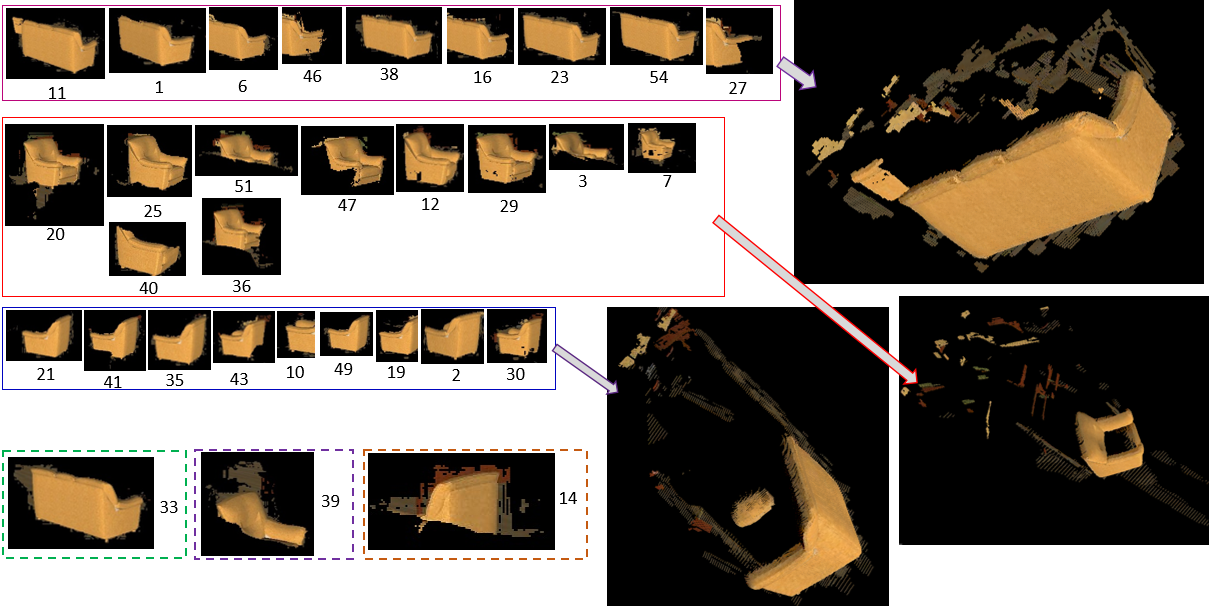
\includegraphics[width=2\columnwidth]{figures/set1/object_set1.png}
	\caption{Object clustering by geometric registration. The solid rectangles indicate that multiple regions are accurately registered. The regions in dashed rectangles can not be aligned to any other objects due to larger registration error. }
	\label{fig:cluster_object_1}
\end{figure*}


\begin{figure*}
	\centering
	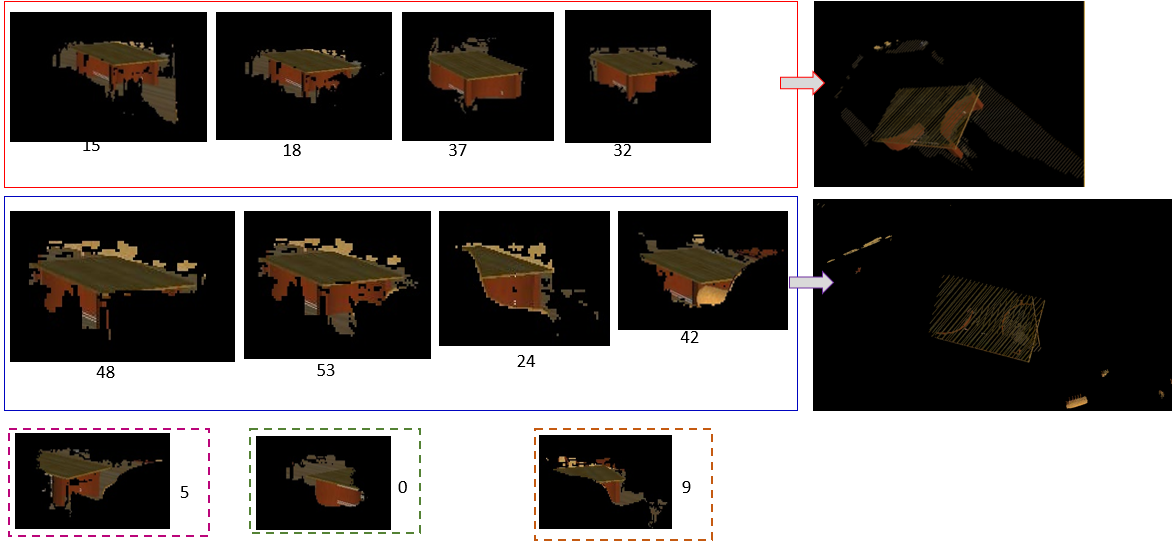
\includegraphics[width=2\columnwidth]{figures/set1/object_set2.png}
	\caption{Object clustering by geometric registration. The solid rectangles indicate that multiple regions are accurately registered. The regions in dashed rectangles can not be aligned to any other objects due to larger registration error. }
	\label{fig:cluster_object_2}
\end{figure*}


\comment{
\begin{figure}
	\centering
	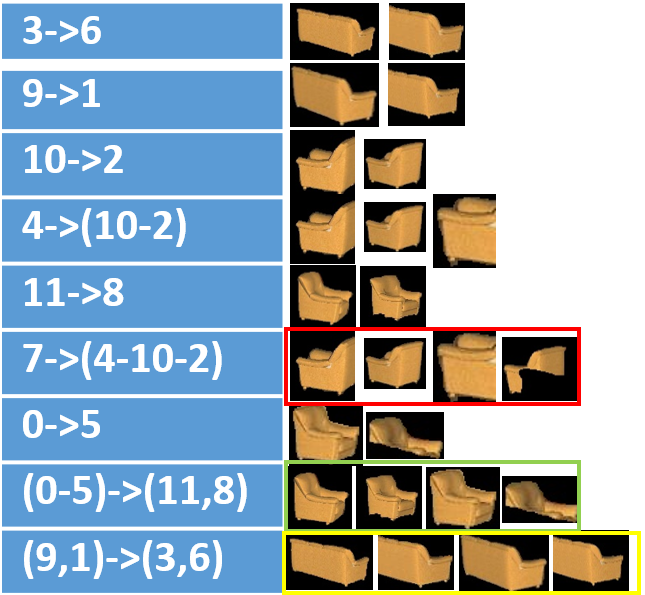
\includegraphics[width=\columnwidth]{figures/set1/grouping.png}
	\caption{\label{fig:seg_object_grouping} Merging segments. Three groups are obtained from 12 segments. The left show all the merging steps. The right show the segments who are merged at each step.  }
\end{figure}

\begin{figure}
	\centering
	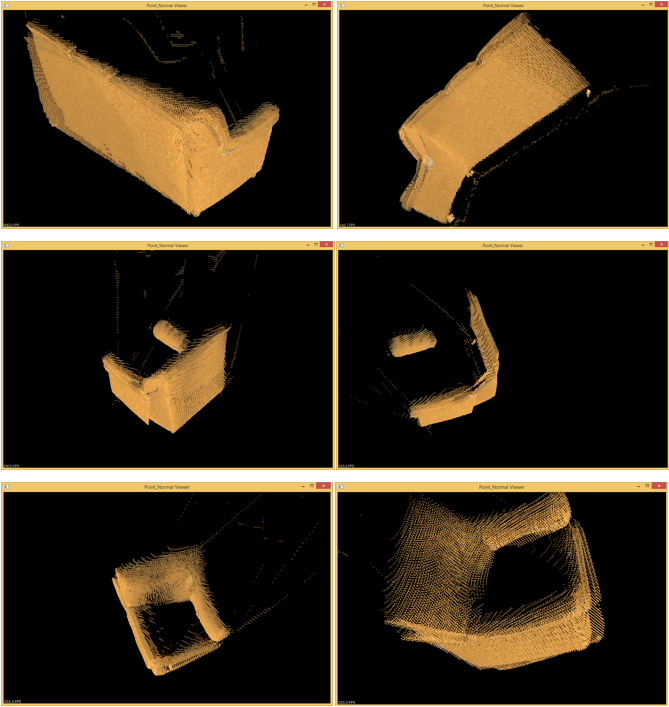
\includegraphics[width=\columnwidth]{figures/set1/object_model.png}
	\caption{\label{fig:object_model} The registered point clouds for the three groups of sofa segments. \redemph{There are still many artifacts on the aligned point clouds.}}
\end{figure}
}
